% interactcadsample.tex
% v1.03 - April 2017

\documentclass[]{interact}

\usepackage{epstopdf}% To incorporate .eps illustrations using PDFLaTeX, etc.
\usepackage{subfigure}% Support for small, `sub' figures and tables
%\usepackage[nolists,tablesfirst]{endfloat}% To `separate' figures and tables from text if required

\usepackage{natbib}% Citation support using natbib.sty
\bibpunct[, ]{(}{)}{;}{a}{}{,}% Citation support using natbib.sty
\renewcommand\bibfont{\fontsize{10}{12}\selectfont}% Bibliography support using natbib.sty

\theoremstyle{plain}% Theorem-like structures provided by amsthm.sty
\newtheorem{theorem}{Theorem}[section]
\newtheorem{lemma}[theorem]{Lemma}
\newtheorem{corollary}[theorem]{Corollary}
\newtheorem{proposition}[theorem]{Proposition}

\theoremstyle{definition}
\newtheorem{definition}[theorem]{Definition}
\newtheorem{example}[theorem]{Example}

\theoremstyle{remark}
\newtheorem{remark}{Remark}
\newtheorem{notation}{Notation}

% Pandoc syntax highlighting
\usepackage{color}
\usepackage{fancyvrb}
\newcommand{\VerbBar}{|}
\newcommand{\VERB}{\Verb[commandchars=\\\{\}]}
\DefineVerbatimEnvironment{Highlighting}{Verbatim}{commandchars=\\\{\}}
% Add ',fontsize=\small' for more characters per line
\usepackage{framed}
\definecolor{shadecolor}{RGB}{248,248,248}
\newenvironment{Shaded}{\begin{snugshade}}{\end{snugshade}}
\newcommand{\AlertTok}[1]{\textcolor[rgb]{0.94,0.16,0.16}{#1}}
\newcommand{\AnnotationTok}[1]{\textcolor[rgb]{0.56,0.35,0.01}{\textbf{\textit{#1}}}}
\newcommand{\AttributeTok}[1]{\textcolor[rgb]{0.77,0.63,0.00}{#1}}
\newcommand{\BaseNTok}[1]{\textcolor[rgb]{0.00,0.00,0.81}{#1}}
\newcommand{\BuiltInTok}[1]{#1}
\newcommand{\CharTok}[1]{\textcolor[rgb]{0.31,0.60,0.02}{#1}}
\newcommand{\CommentTok}[1]{\textcolor[rgb]{0.56,0.35,0.01}{\textit{#1}}}
\newcommand{\CommentVarTok}[1]{\textcolor[rgb]{0.56,0.35,0.01}{\textbf{\textit{#1}}}}
\newcommand{\ConstantTok}[1]{\textcolor[rgb]{0.00,0.00,0.00}{#1}}
\newcommand{\ControlFlowTok}[1]{\textcolor[rgb]{0.13,0.29,0.53}{\textbf{#1}}}
\newcommand{\DataTypeTok}[1]{\textcolor[rgb]{0.13,0.29,0.53}{#1}}
\newcommand{\DecValTok}[1]{\textcolor[rgb]{0.00,0.00,0.81}{#1}}
\newcommand{\DocumentationTok}[1]{\textcolor[rgb]{0.56,0.35,0.01}{\textbf{\textit{#1}}}}
\newcommand{\ErrorTok}[1]{\textcolor[rgb]{0.64,0.00,0.00}{\textbf{#1}}}
\newcommand{\ExtensionTok}[1]{#1}
\newcommand{\FloatTok}[1]{\textcolor[rgb]{0.00,0.00,0.81}{#1}}
\newcommand{\FunctionTok}[1]{\textcolor[rgb]{0.00,0.00,0.00}{#1}}
\newcommand{\ImportTok}[1]{#1}
\newcommand{\InformationTok}[1]{\textcolor[rgb]{0.56,0.35,0.01}{\textbf{\textit{#1}}}}
\newcommand{\KeywordTok}[1]{\textcolor[rgb]{0.13,0.29,0.53}{\textbf{#1}}}
\newcommand{\NormalTok}[1]{#1}
\newcommand{\OperatorTok}[1]{\textcolor[rgb]{0.81,0.36,0.00}{\textbf{#1}}}
\newcommand{\OtherTok}[1]{\textcolor[rgb]{0.56,0.35,0.01}{#1}}
\newcommand{\PreprocessorTok}[1]{\textcolor[rgb]{0.56,0.35,0.01}{\textit{#1}}}
\newcommand{\RegionMarkerTok}[1]{#1}
\newcommand{\SpecialCharTok}[1]{\textcolor[rgb]{0.00,0.00,0.00}{#1}}
\newcommand{\SpecialStringTok}[1]{\textcolor[rgb]{0.31,0.60,0.02}{#1}}
\newcommand{\StringTok}[1]{\textcolor[rgb]{0.31,0.60,0.02}{#1}}
\newcommand{\VariableTok}[1]{\textcolor[rgb]{0.00,0.00,0.00}{#1}}
\newcommand{\VerbatimStringTok}[1]{\textcolor[rgb]{0.31,0.60,0.02}{#1}}
\newcommand{\WarningTok}[1]{\textcolor[rgb]{0.56,0.35,0.01}{\textbf{\textit{#1}}}}

% tightlist command for lists without linebreak
\providecommand{\tightlist}{%
  \setlength{\itemsep}{0pt}\setlength{\parskip}{0pt}}

% From pandoc table feature
\usepackage{longtable,booktabs,array}
\usepackage{calc} % for calculating minipage widths
% Correct order of tables after \paragraph or \subparagraph
\usepackage{etoolbox}
\makeatletter
\patchcmd\longtable{\par}{\if@noskipsec\mbox{}\fi\par}{}{}
\makeatother
% Allow footnotes in longtable head/foot
\IfFileExists{footnotehyper.sty}{\usepackage{footnotehyper}}{\usepackage{footnote}}
\makesavenoteenv{longtable}


\usepackage{hyperref}
\usepackage[utf8]{inputenc}
\def\tightlist{}


\begin{document}


\articletype{PREPRINT}

\title{Exploring Equivalence Testing with the TOSTER R package}


\author{\name{Aaron R. Caldwell$^{a}$}
\affil{$^{a}$Natick, MA, \url{https://orcid.org/0000-0002-4541-6283}}
}

\thanks{CONTACT Aaron R.
Caldwell. Email: \href{mailto:arcaldwell49@gmail.com}{\nolinkurl{arcaldwell49@gmail.com}}}

\maketitle

\begin{abstract}
This is an article detailing the ``avocado TOST'' update to the TOSTER R
package.
\end{abstract}

\begin{keywords}
statistics, bootstrapping, minimal effects test, NHST, TOST
\end{keywords}

\hypertarget{introduction}{%
\section{Introduction}\label{introduction}}

Researchers often erroneously declare that no statistical effect exists
based on a single ``non-significant'' p-value \citep{blandaltman95}. In
many of these cases, the data may corroborate the researchers claim but
the interpretation of a null hypothesis significance test (NHST),
wherein the null hypothesis is ``no effect'', is nonetheless incorrect.
In order to statistically test for whether there is ``no effect'' or
``no difference'' researchers could explore using equivalence testing
(CITE Welleck and Senn books). A very simple equivalence testing
approach is the ``two one-sided tests'' (TOST) procedure
\citep{schuirmann1987}. In the TOST procedure, an upper (\(\Delta_U\))
and lower (\(\Delta_L\)) equivalence bound is specified based on the
smallest effect size of interest (SESOI). If the TOST procedure
indicates the effect is close enough to zero to be practically
equivalent then (CITE Lakens).

Both the complaints about erroneous conclusions regarding equivalence
\citep{blandaltman95} and proposed statistical solutions
\citep{schuirmann1987} have existed for decades now. Yet the problem
appears to persist in many applied disciplines. I estimate that the
cause of this continued dissonance is due to a lack of education on
equivalence testing and struggle for many applied researchers to
implement equivalence testing. In my experience, most researchers have
received some degree of statistical training in their doctoral or
master's studies\footnote{I do not mean to blame educators for this
  problem. I merely want to point out that}, but it is rare that any
have idea of equivalence testing. It may also be difficult to implement
equivalence testing for many researchers. This may be caused by most
statistical software defaulting to a null hypothesis of zero, or even
completely lacking an ability to change the null hypothesis.

The TOSTER R package was orginally developed in 2018 (CITE Lakens) to
introduce experimental psychologists to the concept of equivalence
testing. Since then I have made a significant update to the package in
order to improve the user interface and expand the tools available
within the pacakge. TOSTER (Avocado TOST edition \textgreater v0.4.0) is
a good tool to introduce the idea of equivalence testing to the average
researcher who is already familiar with equivalence testing.

One possible source of this misinterpretation may be due to the fact
that many researchers are

An experienced R programmer may have no problem performing equivalence
testing within R but beginners may struggle with both writing the code
and interpreting the output.

\hypertarget{basics-of-equivalence-testing}{%
\section{Basics of Equivalence
Testing}\label{basics-of-equivalence-testing}}

\hypertarget{the-toster-r-package}{%
\subsection{The TOSTER R Package}\label{the-toster-r-package}}

In an effort to make \texttt{TOSTER} more informative and easier to use,
a new function \texttt{t\_TOST} has been created. This function operates
very similarly to base R's \texttt{t.test} function, but performs 3
t-tests (one two-tailed and two one-tailed tests). In addition, this
function has a generic method where two vectors can be supplied or a
formula can be given (e.g.,\texttt{y\ \textasciitilde{}\ group}). This
function also makes it easier to switch between types of t-tests. All
three types (two sample, one sample, and paired samples) can be
performed/calculated from the same function. Moreover, the summary
information and visualizations have been upgraded. This should make the
decisions derived from the function more informative and user-friendly.

Also, \texttt{t\_TOST} is not limited to equivalence tests. Minimal
effects testing (MET) is possible. MET is useful for situations where
the hypothesis is about a minimal effect and the null hypothesis
\emph{is} equivalence.

\begin{figure}
\centering
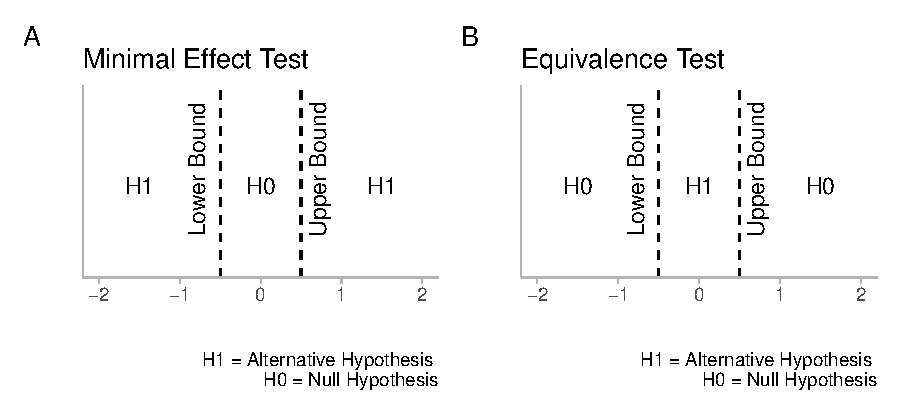
\includegraphics{Avocado_Update_files/figure-latex/hypplot-1.pdf}
\caption{Type of Hypothesis}
\end{figure}

\hypertarget{vignettes-with-toster}{%
\subsection{Vignettes with TOSTER}\label{vignettes-with-toster}}

In the general introduction to this package we detailed how to look at
\emph{old} results and how to apply TOST to interpreting those results.
However, in many cases, users may have new data that needs to be
analyzed. Therefore, \texttt{t\_TOST} can be applied to new data. This
vignette will use the \texttt{bugs} data from the \texttt{jmv} R package
and the \texttt{sleep} data.

\begin{Shaded}
\begin{Highlighting}[]
\FunctionTok{data}\NormalTok{(}\StringTok{\textquotesingle{}sleep\textquotesingle{}}\NormalTok{)}
\FunctionTok{library}\NormalTok{(jmv)}
\FunctionTok{data}\NormalTok{(}\StringTok{\textquotesingle{}bugs\textquotesingle{}}\NormalTok{)}
\end{Highlighting}
\end{Shaded}

\hypertarget{independent-groups}{%
\subsubsection{Independent Groups}\label{independent-groups}}

For this example, we will use the sleep data. In this data there is a
\texttt{group} variable and an outcome \texttt{extra}.

\begin{Shaded}
\begin{Highlighting}[]
\FunctionTok{head}\NormalTok{(sleep)}
\end{Highlighting}
\end{Shaded}

\begin{verbatim}
##   extra group ID
## 1   0.7     1  1
## 2  -1.6     1  2
## 3  -0.2     1  3
## 4  -1.2     1  4
## 5  -0.1     1  5
## 6   3.4     1  6
\end{verbatim}

We will assume the data are independent, and that we have equivalence
bounds of +/- 0.5. All we need to do is provide the \texttt{formula},
\texttt{data}, and eqbound arguments for the function to run
appropriately. In addition, we can set the \texttt{var.equal} argument
(to assume equal variance), and the \texttt{paired} argument (sets if
the data is paired or not). Both are logical indicators that can be set
to TRUE or FALSE. The \texttt{alpha} is automatically set to 0.05 but
this can also be adjusted by the user. The Hedges correction is also
automatically calculated, but this can be overridden with the
\texttt{bias\_correction} argument. The \texttt{hypothesis} is
automatically set to ``EQU'' for equivalence but if a minimal effect is
of interest then ``MET'' can be supplied

\begin{Shaded}
\begin{Highlighting}[]
\CommentTok{\# Formula Interface}
\NormalTok{res1 }\OtherTok{=} \FunctionTok{t\_TOST}\NormalTok{(}\AttributeTok{formula =}\NormalTok{ extra }\SpecialCharTok{\textasciitilde{}}\NormalTok{ group,}
              \AttributeTok{data =}\NormalTok{ sleep,}
              \AttributeTok{low\_eqbound =} \SpecialCharTok{{-}}\NormalTok{.}\DecValTok{5}\NormalTok{,}
              \AttributeTok{high\_eqbound =}\NormalTok{ .}\DecValTok{5}\NormalTok{)}

\CommentTok{\# x \& y interface}
\NormalTok{res1a }\OtherTok{=} \FunctionTok{t\_TOST}\NormalTok{(}\AttributeTok{x =} \FunctionTok{subset}\NormalTok{(sleep,group}\SpecialCharTok{==}\DecValTok{1}\NormalTok{)}\SpecialCharTok{$}\NormalTok{extra,}
               \AttributeTok{y =} \FunctionTok{subset}\NormalTok{(sleep,group}\SpecialCharTok{==}\DecValTok{2}\NormalTok{)}\SpecialCharTok{$}\NormalTok{extra,}
               \AttributeTok{low\_eqbound =} \SpecialCharTok{{-}}\NormalTok{.}\DecValTok{5}\NormalTok{,}
               \AttributeTok{high\_eqbound =}\NormalTok{ .}\DecValTok{5}\NormalTok{)}
\end{Highlighting}
\end{Shaded}

Once the function has run, we can print the results with the
\texttt{print} command. This provides a verbose summary of the results.

\begin{Shaded}
\begin{Highlighting}[]
\FunctionTok{print}\NormalTok{(res1)}
\end{Highlighting}
\end{Shaded}

\begin{verbatim}
## 
## Welch Two Sample t-test
## Hypothesis Tested: Equivalence
## Equivalence Bounds (raw):-0.500 & 0.500
## Alpha Level:0.05
## The equivalence test was non-significant, t(17.78) = -1.272, p = 8.9e-01
## The null hypothesis test was non-significant, t(17.78) = -1.861, p = 7.94e-02
## NHST: don't reject null significance hypothesis that the effect is equal to zero 
##  TOST: don't reject null equivalence hypothesis
## 
## TOST Results 
##                    t       SE       df    p.value
## t-test     -1.860813 0.849091 17.77647 0.07939414
## TOST Lower -1.271948 0.849091 17.77647 0.89010996
## TOST Upper -2.449678 0.849091 17.77647 0.01245133
## 
## Effect Sizes 
##                 estimate       SE  lower.ci    upper.ci conf.level
## Raw           -1.5800000 0.849091 -3.053381 -0.10661850        0.9
## Hedges' g(av) -0.7964846 0.497633 -1.684326 -0.06154947        0.9
## 
## Note: SMD confidence intervals are an approximation. See vignette("SMD_calcs").
\end{verbatim}

Another nice feature is the generic \texttt{plot} method that can
provide a visual summary of the results. All of the plots in this
package were inspired by the
\href{https://cran.r-project.org/package=concurve}{concurve} R package.
There are two types of plots that can be produced. The first, and
default, is the consonance density plot (\texttt{type\ =\ "cd"}).

\begin{Shaded}
\begin{Highlighting}[]
\FunctionTok{plot}\NormalTok{(res1, }\AttributeTok{type =} \StringTok{"cd"}\NormalTok{)}
\end{Highlighting}
\end{Shaded}

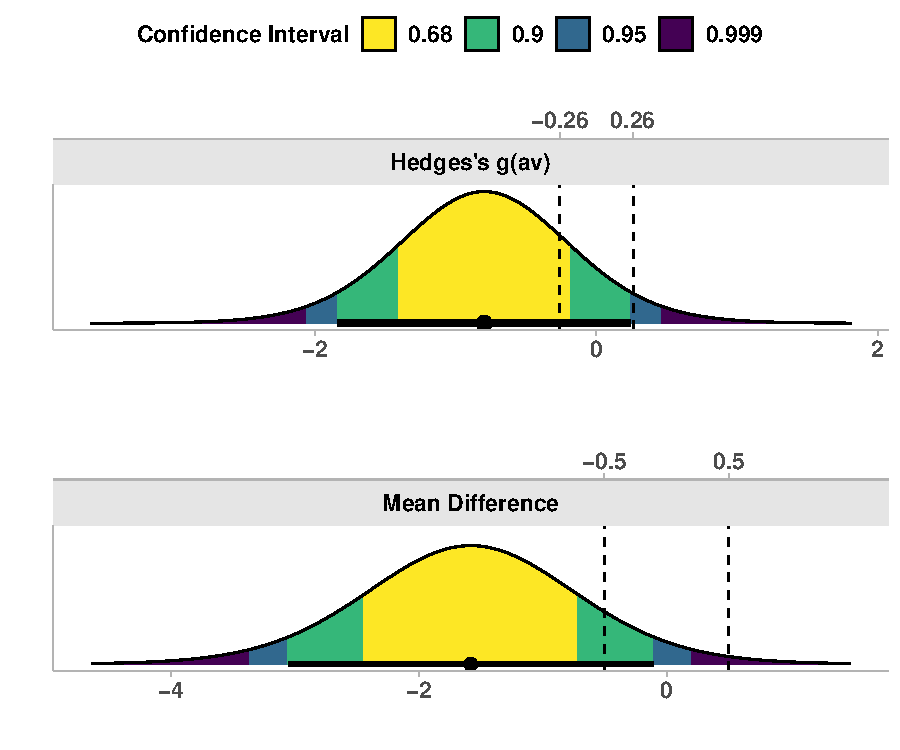
\includegraphics{Avocado_Update_files/figure-latex/unnamed-chunk-5-1.pdf}

The shading pattern can be modified with the \texttt{ci\_shades}.

\begin{Shaded}
\begin{Highlighting}[]
\FunctionTok{plot}\NormalTok{(res1, }\AttributeTok{type =} \StringTok{"cd"}\NormalTok{,}
     \AttributeTok{ci\_shades =} \FunctionTok{c}\NormalTok{(.}\DecValTok{9}\NormalTok{,.}\DecValTok{95}\NormalTok{))}
\end{Highlighting}
\end{Shaded}

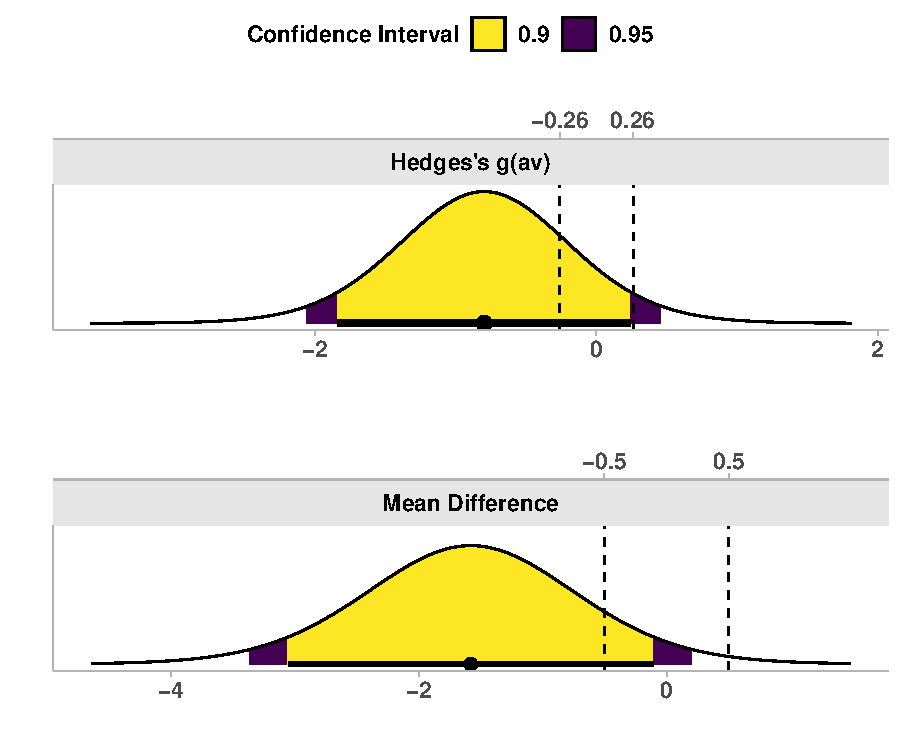
\includegraphics{Avocado_Update_files/figure-latex/unnamed-chunk-6-1.pdf}

Consonance plots, where all confidence intervals can be simultaneous
plotted, can also be produced. The advantage here is multiple confidence
interval lines can plotted at once.

\begin{Shaded}
\begin{Highlighting}[]
\FunctionTok{plot}\NormalTok{(res1, }\AttributeTok{type =} \StringTok{"c"}\NormalTok{,}
     \AttributeTok{ci\_lines =}  \FunctionTok{c}\NormalTok{(.}\DecValTok{9}\NormalTok{,.}\DecValTok{95}\NormalTok{))}
\end{Highlighting}
\end{Shaded}

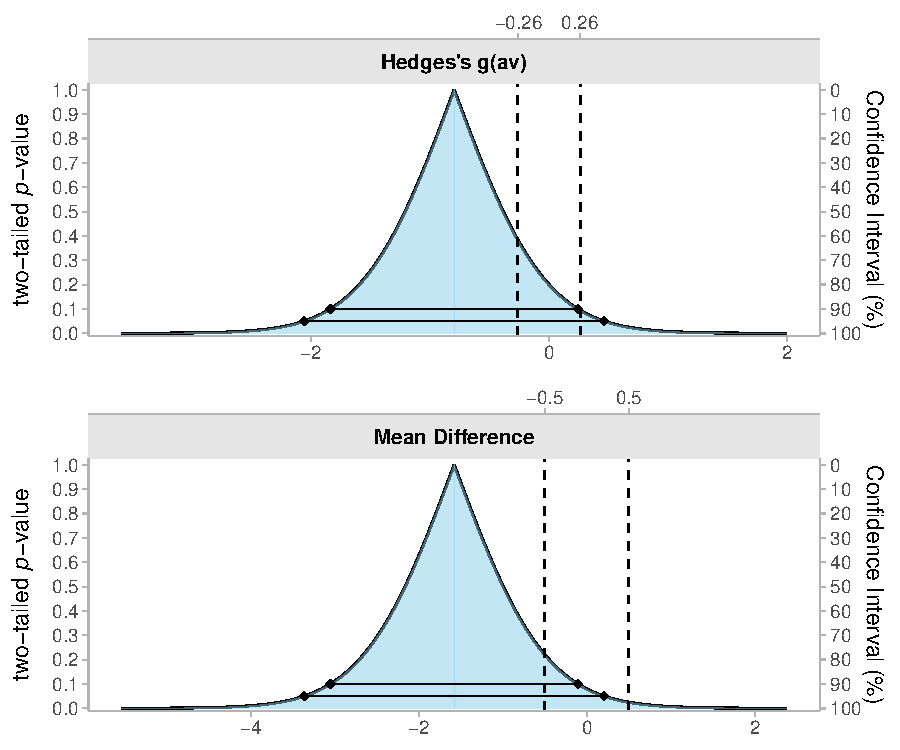
\includegraphics{Avocado_Update_files/figure-latex/unnamed-chunk-7-1.pdf}

\hypertarget{paired-samples}{%
\subsubsection{Paired Samples}\label{paired-samples}}

To perform a paired samples TOST, the process does not change much. We
could process the test the same way by providing a formula. All we would
need to then is change \texttt{paired} to TRUE.

\begin{Shaded}
\begin{Highlighting}[]
\NormalTok{res2 }\OtherTok{=} \FunctionTok{t\_TOST}\NormalTok{(}\AttributeTok{formula =}\NormalTok{ extra }\SpecialCharTok{\textasciitilde{}}\NormalTok{ group,}
              \AttributeTok{data =}\NormalTok{ sleep,}
              \AttributeTok{paired =} \ConstantTok{TRUE}\NormalTok{,}
              \AttributeTok{low\_eqbound =} \SpecialCharTok{{-}}\NormalTok{.}\DecValTok{5}\NormalTok{,}
              \AttributeTok{high\_eqbound =}\NormalTok{ .}\DecValTok{5}\NormalTok{)}
\NormalTok{res2}
\end{Highlighting}
\end{Shaded}

\begin{verbatim}
## 
## Paired t-test
## Hypothesis Tested: Equivalence
## Equivalence Bounds (raw):-0.500 & 0.500
## Alpha Level:0.05
## The equivalence test was non-significant, t(9) = -2.777, p = 9.89e-01
## The null hypothesis test was significant, t(9) = -4.062, p = 2.83e-03
## NHST: reject null significance hypothesis that the effect is equal to zero 
##  TOST: don't reject null equivalence hypothesis
## 
## TOST Results 
##                    t        SE df      p.value
## t-test     -4.062128 0.3889587  9 0.0028328902
## TOST Lower -2.776644 0.3889587  9 0.9892407566
## TOST Upper -5.347611 0.3889587  9 0.0002319027
## 
## Effect Sizes 
##               estimate        SE  lower.ci   upper.ci conf.level
## Raw          -1.580000 0.3889587 -2.293005 -0.8669947        0.9
## Hedges' g(z) -1.230152 0.2008070 -1.848296 -0.8362302        0.9
## 
## Note: SMD confidence intervals are an approximation. See vignette("SMD_calcs").
\end{verbatim}

However, we may have two vectors of data that are paired. So instead we
may want to just provide those separately rather than using a data set
and setting the formula. This can be demonstrated with the ``bugs''
data.

\begin{Shaded}
\begin{Highlighting}[]
\NormalTok{res3 }\OtherTok{=} \FunctionTok{t\_TOST}\NormalTok{(}\AttributeTok{x =}\NormalTok{ bugs}\SpecialCharTok{$}\NormalTok{LDHF,}
              \AttributeTok{y =}\NormalTok{ bugs}\SpecialCharTok{$}\NormalTok{LDLF,}
              \AttributeTok{paired =} \ConstantTok{TRUE}\NormalTok{,}
              \AttributeTok{low\_eqbound =} \SpecialCharTok{{-}}\DecValTok{1}\NormalTok{,}
              \AttributeTok{high\_eqbound =} \DecValTok{1}\NormalTok{)}
\NormalTok{res3}
\end{Highlighting}
\end{Shaded}

\begin{verbatim}
## 
## Paired t-test
## Hypothesis Tested: Equivalence
## Equivalence Bounds (raw):-1.000 & 1.000
## Alpha Level:0.05
## The equivalence test was non-significant, t(90) = 2.655, p = 9.95e-01
## The null hypothesis test was significant, t(90) = 6.649, p = 2.22e-09
## NHST: reject null significance hypothesis that the effect is equal to zero 
##  TOST: don't reject null equivalence hypothesis
## 
## TOST Results 
##                    t        SE df      p.value
## t-test      6.648618 0.2504032 90 2.223690e-09
## TOST Lower 10.642177 0.2504032 90 6.681389e-18
## TOST Upper  2.655058 0.2504032 90 9.953114e-01
## 
## Effect Sizes 
##               estimate         SE  lower.ci  upper.ci conf.level
## Raw          1.6648352 0.25040321 1.2486748 2.0809956        0.9
## Hedges' g(z) 0.6940558 0.09548981 0.5296194 0.8707979        0.9
## 
## Note: SMD confidence intervals are an approximation. See vignette("SMD_calcs").
\end{verbatim}

We may want to perform a Minimal Effect Test with the
\texttt{hypothesis} argument set to ``MET''.

\begin{Shaded}
\begin{Highlighting}[]
\NormalTok{res3a }\OtherTok{=} \FunctionTok{t\_TOST}\NormalTok{(}\AttributeTok{x =}\NormalTok{ bugs}\SpecialCharTok{$}\NormalTok{LDHF,}
               \AttributeTok{y =}\NormalTok{ bugs}\SpecialCharTok{$}\NormalTok{LDLF,}
               \AttributeTok{paired =} \ConstantTok{TRUE}\NormalTok{,}
               \AttributeTok{hypothesis =} \StringTok{"MET"}\NormalTok{,}
               \AttributeTok{low\_eqbound =} \SpecialCharTok{{-}}\DecValTok{1}\NormalTok{,}
               \AttributeTok{high\_eqbound =} \DecValTok{1}\NormalTok{)}
\NormalTok{res3a}
\end{Highlighting}
\end{Shaded}

\begin{verbatim}
## 
## Paired t-test
## Hypothesis Tested: Minimal Effect
## Equivalence Bounds (raw):-1.000 & 1.000
## Alpha Level:0.05
## The minimal effect test was significant, t(90) = 10.642, p = 4.69e-03
## The null hypothesis test was significant, t(90) = 6.649, p = 2.22e-09
## NHST: reject null significance hypothesis that the effect is equal to zero 
##  TOST: reject null MET hypothesis
## 
## TOST Results 
##                    t        SE df      p.value
## t-test      6.648618 0.2504032 90 2.223690e-09
## TOST Lower 10.642177 0.2504032 90 1.000000e+00
## TOST Upper  2.655058 0.2504032 90 4.688649e-03
## 
## Effect Sizes 
##               estimate         SE  lower.ci  upper.ci conf.level
## Raw          1.6648352 0.25040321 1.2486748 2.0809956        0.9
## Hedges' g(z) 0.6940558 0.09548981 0.5296194 0.8707979        0.9
## 
## Note: SMD confidence intervals are an approximation. See vignette("SMD_calcs").
\end{verbatim}

Again, we can plot the effects from the \texttt{t\_TOST} result.

\begin{Shaded}
\begin{Highlighting}[]
\FunctionTok{plot}\NormalTok{(res3a)}
\end{Highlighting}
\end{Shaded}

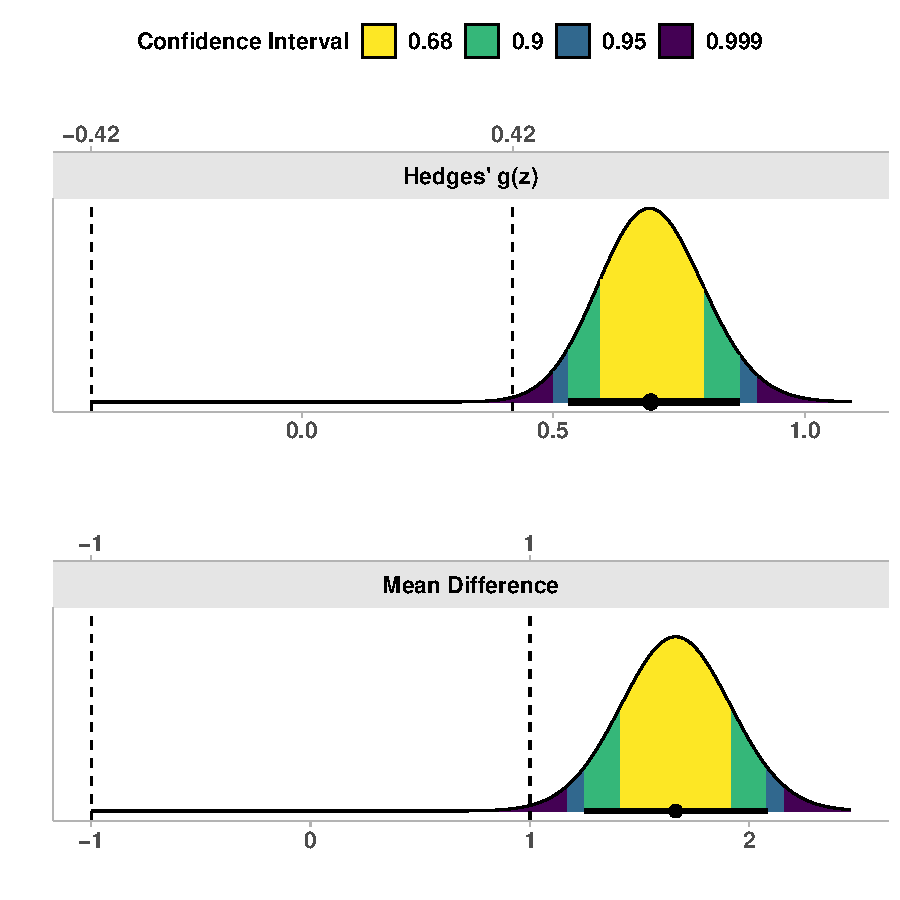
\includegraphics{Avocado_Update_files/figure-latex/unnamed-chunk-11-1.pdf}

\hypertarget{one-sample-t-test}{%
\subsubsection{One Sample t-test}\label{one-sample-t-test}}

In other cases we may just have a one sample test. If that is the case
all we have to do is supply the \texttt{x} argument for the data. For
this test we may hypothesis that the mean of LDHF is not more than 1.5
points greater or less than 7.

\begin{Shaded}
\begin{Highlighting}[]
\NormalTok{res4 }\OtherTok{=} \FunctionTok{t\_TOST}\NormalTok{(}\AttributeTok{x =}\NormalTok{ bugs}\SpecialCharTok{$}\NormalTok{LDHF,}
              \AttributeTok{hypothesis =} \StringTok{"EQU"}\NormalTok{,}
              \AttributeTok{low\_eqbound =} \FloatTok{5.5}\NormalTok{,}
              \AttributeTok{high\_eqbound =} \FloatTok{8.5}\NormalTok{)}
\NormalTok{res4}
\end{Highlighting}
\end{Shaded}

\begin{verbatim}
## 
## One Sample t-test
## Hypothesis Tested: Equivalence
## Equivalence Bounds (raw):5.500 & 8.500
## Alpha Level:0.05
## The equivalence test was significant, t(90) = -4.244, p = 2.66e-05
## The null hypothesis test was significant, t(90) = 27.942, p = 3.91e-46
## NHST: reject null significance hypothesis that the effect is equal to zero 
## TOST: reject null equivalence hypothesis
## 
## TOST Results 
##                    t        SE df      p.value
## t-test     27.942403 0.2640833 90 3.906969e-46
## TOST Lower  7.115638 0.2640833 90 1.298575e-10
## TOST Upper -4.244416 0.2640833 90 2.658068e-05
## 
## Effect Sizes 
##           estimate        SE lower.ci upper.ci conf.level
## Raw       7.379121 0.2640833 6.940225 7.818017        0.9
## Hedges' g 2.904671 0.2452067 2.551811 3.354884        0.9
## 
## Note: SMD confidence intervals are an approximation. See vignette("SMD_calcs").
\end{verbatim}

\begin{Shaded}
\begin{Highlighting}[]
\FunctionTok{plot}\NormalTok{(res4)}
\end{Highlighting}
\end{Shaded}

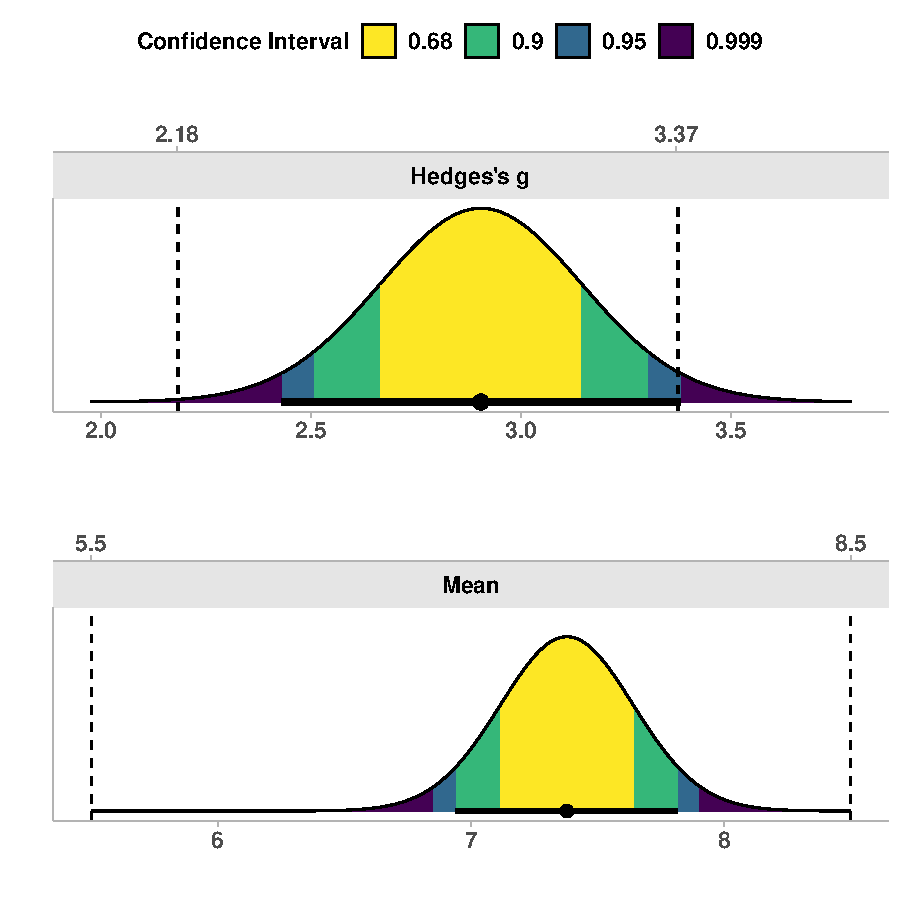
\includegraphics{Avocado_Update_files/figure-latex/unnamed-chunk-13-1.pdf}

\hypertarget{using-summary-statistics}{%
\subsubsection{Using Summary
Statistics}\label{using-summary-statistics}}

In some cases you may only have access to the summary statistics.
Therefore, we created a function, \texttt{tsum\_TOST},to perform the
same tests just based on the summary statistics. This involves providing
the function with a number of different arguments.

\begin{itemize}
\tightlist
\item
  \texttt{n1\ \&\ n2} the sample sizes (only n1 needs to be provided for
  one sample case)
\item
  \texttt{m1\ \&\ m2} the sample means
\item
  \texttt{sd1\ \&\ sd2} the sample standard deviation
\item
  \texttt{r12} the correlation between each if paired is set to TRUE
\end{itemize}

The results from above can be replicated with the \texttt{tsum\_TOST}

\begin{Shaded}
\begin{Highlighting}[]
\NormalTok{res\_tsum }\OtherTok{=} \FunctionTok{tsum\_TOST}\NormalTok{(}
  \AttributeTok{m1 =} \FunctionTok{mean}\NormalTok{(bugs}\SpecialCharTok{$}\NormalTok{LDHF, }\AttributeTok{na.rm=}\ConstantTok{TRUE}\NormalTok{),}
  \AttributeTok{sd1 =} \FunctionTok{sd}\NormalTok{(bugs}\SpecialCharTok{$}\NormalTok{LDHF, }\AttributeTok{na.rm=}\ConstantTok{TRUE}\NormalTok{),}
  \AttributeTok{n1 =} \FunctionTok{length}\NormalTok{(}\FunctionTok{na.omit}\NormalTok{(bugs}\SpecialCharTok{$}\NormalTok{LDHF)),}
  \AttributeTok{hypothesis =} \StringTok{"EQU"}\NormalTok{,}
  \AttributeTok{low\_eqbound =} \FloatTok{5.5}\NormalTok{,}
  \AttributeTok{high\_eqbound =} \FloatTok{8.5}
\NormalTok{)}

\NormalTok{res\_tsum}
\end{Highlighting}
\end{Shaded}

\begin{verbatim}
## 
## One-sample t-Test
## Hypothesis Tested: Equivalence
## Equivalence Bounds (raw):5.500 & 8.500
## Alpha Level:0.05
## The equivalence test was significant, t(90) = -4.244, p = 2.66e-05
## The null hypothesis test was significant, t(90) = 27.942, p = 3.91e-46
## NHST: reject null significance hypothesis that the effect is equal to zero 
## TOST: reject null equivalence hypothesis
## 
## TOST Results 
##                    t        SE df      p.value
## t-test     27.942403 0.2640833 90 3.906969e-46
## TOST Lower  7.115638 0.2640833 90 1.298575e-10
## TOST Upper -4.244416 0.2640833 90 2.658068e-05
## 
## Effect Sizes 
##           estimate        SE lower.ci upper.ci conf.level
## Raw       7.379121 0.2640833 6.940225 7.818017        0.9
## Hedges' g 2.904671 0.2452067 2.551811 3.354884        0.9
## 
## Note: SMD confidence intervals are an approximation. See vignette("SMD_calcs").
\end{verbatim}

\begin{Shaded}
\begin{Highlighting}[]
\FunctionTok{plot}\NormalTok{(res\_tsum)}
\end{Highlighting}
\end{Shaded}

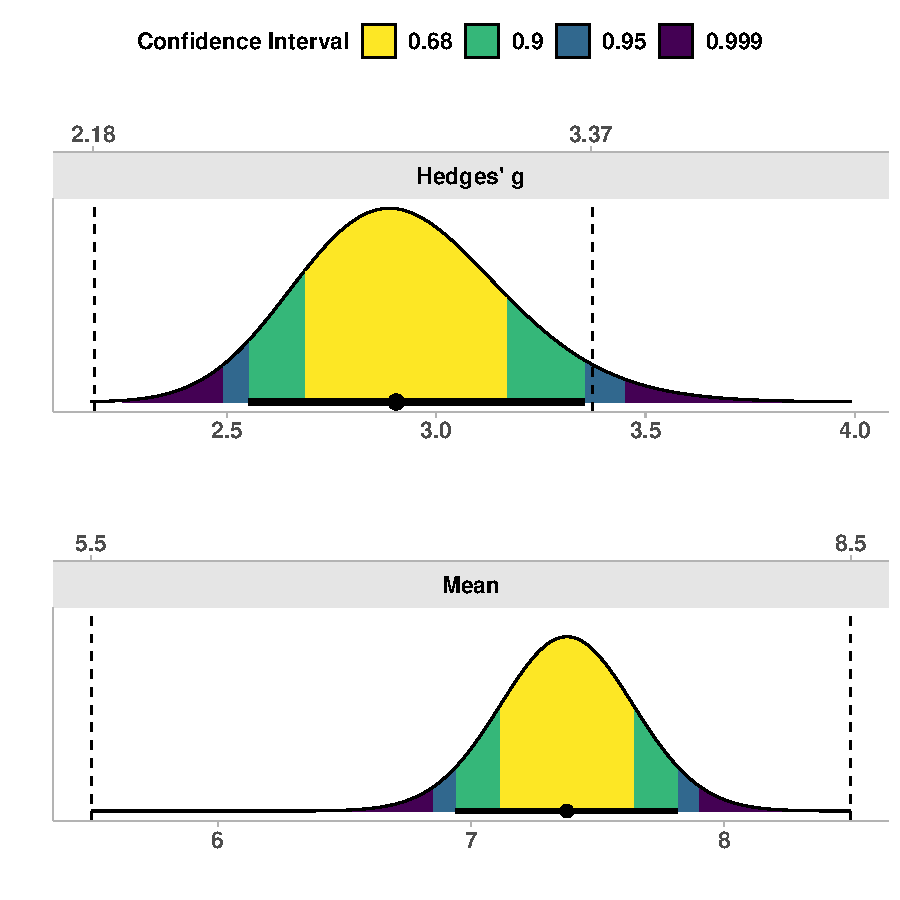
\includegraphics{Avocado_Update_files/figure-latex/unnamed-chunk-15-1.pdf}

\hypertarget{robust-methods-for-equivalence-testing}{%
\section{Robust Methods for Equivalence
Testing}\label{robust-methods-for-equivalence-testing}}

Why this may be useful Describe these aren't tests of medians but
symmetry tests (myth busting) Paired samples may want to be rank
transformed

In this package there are currently 2 functions that provide robust
alternatives to the \texttt{t\_TOST} function.

\hypertarget{tests-of-symmetry}{%
\subsection{Tests of Symmetry}\label{tests-of-symmetry}}

The Wilcoxon group of tests (includes Mann-Whitney U-test) provide a
non-parametric test of differences between groups, or within samples,
based on ranks. This provides a test of location shift, which is a fancy
way of saying differences in the center of the distribution (i.e., in
parametric tests the location is mean). With TOST, there are two
separate tests of directional location shift to determine if the
location shift is within (equivalence) or outside (minimal effect). The
exact calculations can be explored via the documentation of the
\texttt{wilcox.test} function.

In the TOSTER package, we accomplish this with the \texttt{wilcox\_TOST}
function. Overall, this function operates extremely similar to the
\texttt{t\_TOST} function. However, the standardized mean difference
(SMD) is \emph{not} calculated. Instead the rank-biserial correlation is
calculated for \emph{all} types of comparisons (e.g., two sample, one
sample, and paired samples). Also, there is no plotting capability at
this time for the output of this function.

As an example, we can use the sleep data to make a non-parametric
comparison of equivalence.

\begin{Shaded}
\begin{Highlighting}[]
\FunctionTok{data}\NormalTok{(}\StringTok{\textquotesingle{}sleep\textquotesingle{}}\NormalTok{)}
\FunctionTok{library}\NormalTok{(TOSTER)}

\NormalTok{test1 }\OtherTok{=} \FunctionTok{wilcox\_TOST}\NormalTok{(}\AttributeTok{formula =}\NormalTok{ extra }\SpecialCharTok{\textasciitilde{}}\NormalTok{ group,}
                      \AttributeTok{data =}\NormalTok{ sleep,}
                      \AttributeTok{paired =} \ConstantTok{FALSE}\NormalTok{,}
                      \AttributeTok{low\_eqbound =} \SpecialCharTok{{-}}\NormalTok{.}\DecValTok{5}\NormalTok{,}
                      \AttributeTok{high\_eqbound =}\NormalTok{ .}\DecValTok{5}\NormalTok{)}


\FunctionTok{print}\NormalTok{(test1)}
\end{Highlighting}
\end{Shaded}

\begin{verbatim}
## 
## Wilcoxon rank sum test with continuity correction
## Hypothesis Tested: Equivalence
## Equivalence Bounds (raw):-0.500 & 0.500
## Alpha Level:0.05
## The equivalence test was non-significant W = 20.000, p = 8.94e-01
## The null hypothesis test was non-significant W = 25.500, p = 6.93e-02
## NHST: don't reject null significance hypothesis that the effect is equal to zero 
## TOST: don't reject null equivalence hypothesis
## 
## TOST Results 
##            statistic    p.value
## NHST            25.5 0.06932758
## TOST Lower      34.0 0.89385308
## TOST Upper      20.0 0.01287404
## 
## Effect Sizes 
##                            estimate   lower.ci    upper.ci conf.level
## Median of Differences     -1.346388 -3.3999651 -0.09995341        0.9
## rank-biserial correlation -0.490000 -0.7492521 -0.10053222        0.9
\end{verbatim}

\hypertarget{boostrap-tost}{%
\subsection{Boostrap TOST}\label{boostrap-tost}}

The boostrap refers to resampling with replacement and can be used
statistical estimation and inference. Bootsrapping techniques are very
useful because they are considered somewhat robust to the violations of
assumptions for a simple t-test. Therefore we added a bootstrap option,
\texttt{boot\_t\_TOST} to the package to provide another robust
alternative to the \texttt{t\_TOST} function.

In this function we provide a percentile bootstrap solution outlined by
\citet{efron93} (see chapter 16, page 220). The bootstrapped p-values
are derived from the ``studentized'' version of a test of mean
differences \citep{efron93}. Overall, the results should be similar to
the results of \texttt{t\_TOST}. \textbf{However}, for paired samples,
the Cohen's d(rm) effect size \emph{cannot} be calculated at this time.

\hypertarget{two-sample-algorithm}{%
\subsubsection{Two Sample Algorithm}\label{two-sample-algorithm}}

\begin{enumerate}
\def\labelenumi{\arabic{enumi}.}
\item
  Form B bootstrap data sets from x* and y* wherein x* is sampled with
  replacement from \(\tilde x_1,\tilde x_2, ... \tilde x_n\) and y* is
  sampled with replacement from
  \(\tilde y_1,\tilde y_2, ... \tilde y_n\)
\item
  t is then evaluated on each sample, but the mean of each sample (y or
  x) and the overall average (z) are subtracted from each
\end{enumerate}

\[
t(z^{*b}) = \frac {(\bar x^*-\bar x - \bar z) - (\bar y^*-\bar y - \bar z)}{\sqrt {sd_y^*/n_y + sd_x^*/n_x}}
\]

\begin{enumerate}
\def\labelenumi{\arabic{enumi}.}
\setcounter{enumi}{2}
\tightlist
\item
  An approximate p-value can then be calculated as the number of
  bootstrapped results greater than the observed t-statistic from the
  sample.
\end{enumerate}

\[
p_{boot} = \frac {\#t(z^{*b}) \ge t_{sample}}{B}
\]

The same process is completed for the one sample case but with the one
sample solution for the equation outlined by \(t(z^{*b})\). The paired
sample case in this bootstrap procedure is equivalent to the one sample
solution because the test is based on the difference scores.

\hypertarget{example-of-bootrapping}{%
\subsubsection{Example of Bootrapping}\label{example-of-bootrapping}}

Again, we can use the sleep data to see the bootstrapped results. Notice
that the plots show how the resampling via boostrapping indicates the
instability of Hedges' d(z).

\begin{Shaded}
\begin{Highlighting}[]
\FunctionTok{data}\NormalTok{(}\StringTok{\textquotesingle{}sleep\textquotesingle{}}\NormalTok{)}

\NormalTok{test1 }\OtherTok{=} \FunctionTok{boot\_t\_TOST}\NormalTok{(}\AttributeTok{formula =}\NormalTok{ extra }\SpecialCharTok{\textasciitilde{}}\NormalTok{ group,}
                    \AttributeTok{data =}\NormalTok{ sleep,}
                    \AttributeTok{paired =} \ConstantTok{TRUE}\NormalTok{,}
                    \AttributeTok{low\_eqbound =} \SpecialCharTok{{-}}\NormalTok{.}\DecValTok{5}\NormalTok{,}
                    \AttributeTok{high\_eqbound =}\NormalTok{ .}\DecValTok{5}\NormalTok{,}
                    \AttributeTok{R =} \DecValTok{999}\NormalTok{)}


\FunctionTok{print}\NormalTok{(test1)}
\end{Highlighting}
\end{Shaded}

\begin{verbatim}
## 
## Bootstrapped Paired t-test
## Hypothesis Tested: Equivalence
## Equivalence Bounds (raw):-0.500 & 0.500
## Alpha Level:0.05
## The equivalence test was non-significant, t(9) = -2.777, p = 1e+00
## The null hypothesis test was significant, t(9) = -4.062, p = 0e+00
## NHST: reject null significance hypothesis that the effect is equal to zero 
## TOST: don't reject null equivalence hypothesis
## 
## TOST Results 
##                    t        SE df p.value
## t-test     -4.062128 0.3889587  9       0
## TOST Lower -2.776644 0.3889587  9       1
## TOST Upper -5.347611 0.3889587  9       0
## 
## Effect Sizes 
##               estimate        SE  lower.ci   upper.ci conf.level
## Raw          -1.580000 0.3498821 -2.170000 -1.0490000        0.9
## Hedges' g(z) -1.230152 0.7258598 -2.881678 -0.9220578        0.9
## 
## Note: percentile boostrap method utilized.
\end{verbatim}

\hypertarget{equivalence-testing-with-anovas}{%
\section{Equivalence Testing with
ANOVAs}\label{equivalence-testing-with-anovas}}

For an open access tutorial paper explaining how to set equivalence
bounds, and how to perform and report equivalence for ANOVA models see
\citet{Campbell_2021}. These functions are meant to be omnibus tests,
and additional testing may be necessary. For example, comparison of the
estimated marginal means, in addition to or as an alternative of with
may be prudent.

\hypertarget{f-test-calculations}{%
\subsection{F-test Calculations}\label{f-test-calculations}}

Statistical equivalence testing (or ``omnibus non-inferiority testing''
as \citet{Campbell_2021}) for \emph{F}-tests are special use case of the
cumulative distribution function of the non-central \emph{F}
distribution. As \citet{Campbell_2021} state, these type of questions
answer the question: ``Can we reject the hypothesis that the total
proportion of variance in outcome Y attributable to X is greater than or
equal to the equivalence bound \(\Delta\)?''

\[
H_0: \space 1 > \eta^2_p \geq \Delta
\\
H_1: \space 0 \geq \eta^2_p < \Delta
\]

In \texttt{TOSTER} we go a tad farther and calculate a more
generalizable non-centrality parameter that allows the equivalence test
for \emph{F}-tests to be applied to variety of designs.

\citet{Campbell_2021} calculate the \emph{p}-value as:

\[
p = p_f(F; J-1, N-J, \frac{N \cdot \Delta}{1-\Delta})
\]

However, this approach could not be applied to factorial ANOVA and the
paper only outlines how to apply this approach to a one-way ANOVA and an
extension to Welch's one-way ANOVA.

However, the non-centrality parameter (ncp = \(\lambda\)) can be
calculated with the equivalence bound and the degrees of freedom:

\[
\lambda_{eq} = \frac{\Delta}{1-\Delta} \cdot(df_1 + df_2 +1)
\]

The \emph{p}-value for the equivalence test (\(p_{eq}\)) could then be
calculated from traditional ANOVA results and the distribution function:

\[
p_{eq} = p_f(F; df_1, df_2, \lambda_{eq})
\]

\hypertarget{example-of-equivalence-anova-test}{%
\subsection{Example of Equivalence ANOVA
Test}\label{example-of-equivalence-anova-test}}

Using the \texttt{InsectSprays} data set in R and the base R
\texttt{aov} function we can demonstrate how this omnibus equivalence
testing can be applied with \texttt{TOSTER}.

From the initial analysis we an see a clear ``significant'' effect (the
p-value listed is zero but it just very small) of the factor spray.
However, we \emph{may} be interested in testing if the effect is
practically equivalent. I will arbitrarily set the equivalence bound to
a partial eta-squared of 0.35 (\(H_0: \eta^2_p > 0.35\))

\begin{Shaded}
\begin{Highlighting}[]
\FunctionTok{library}\NormalTok{(TOSTER)}
\CommentTok{\# Get Data}
\FunctionTok{data}\NormalTok{(}\StringTok{"InsectSprays"}\NormalTok{)}
\CommentTok{\# Build ANOVA}
\NormalTok{aovtest }\OtherTok{=} \FunctionTok{aov}\NormalTok{(count }\SpecialCharTok{\textasciitilde{}}\NormalTok{ spray,}
              \AttributeTok{data =}\NormalTok{ InsectSprays)}

\CommentTok{\# Display overall results}
\NormalTok{knitr}\SpecialCharTok{::}\FunctionTok{kable}\NormalTok{(broom}\SpecialCharTok{::}\FunctionTok{tidy}\NormalTok{(aovtest),}
            \AttributeTok{caption =} \StringTok{"Traditional ANOVA Test"}\NormalTok{)}
\end{Highlighting}
\end{Shaded}

\begin{longtable}[]{@{}lrrrrr@{}}
\caption{Traditional ANOVA Test}\tabularnewline
\toprule
term & df & sumsq & meansq & statistic & p.value \\
\midrule
\endfirsthead
\toprule
term & df & sumsq & meansq & statistic & p.value \\
\midrule
\endhead
spray & 5 & 2668.833 & 533.76667 & 34.70228 & 0 \\
Residuals & 66 & 1015.167 & 15.38131 & NA & NA \\
\bottomrule
\end{longtable}

We can then use the information in the table above to perform an
equivalence test using the \texttt{equ\_ftest} function. This function
returns an object of the S3 class \texttt{htest} and the output will
look very familiar to the the t-test. The main difference is the
estimates, and confidence interval, are for partial \(\eta^2_p\).

\begin{Shaded}
\begin{Highlighting}[]
\FunctionTok{equ\_ftest}\NormalTok{(}\AttributeTok{Fstat =} \FloatTok{34.70228}\NormalTok{,}
          \AttributeTok{df1 =} \DecValTok{5}\NormalTok{,}
          \AttributeTok{df2 =} \DecValTok{66}\NormalTok{,}
          \AttributeTok{eqbound =} \FloatTok{0.35}\NormalTok{)}
\end{Highlighting}
\end{Shaded}

\begin{verbatim}
## 
##  Equivalence Test from F-test
## 
## data:  Summary Statistics
## F = 34.702, df1 = 5, df2 = 66, p-value = 1
## 95 percent confidence interval:
##  0.5806263 0.7804439
## sample estimates:
## [1] 0.724439
\end{verbatim}

Based on the results above we would conclude there is a significant
effect of ``spray'' and the differences due to spray are \emph{not}
statistically equivalent. In essence, we reject the traditional null
hypothesis of ``no effect'' but accept the null hypothesis of the
equivalence test.

The \texttt{equ\_ftest} is very useful because all you need is very
basic summary statistics. However, if you are doing all your analyses in
R then you can use the \texttt{equ\_anova} function. This function
accepts objects produced from \texttt{stats::aov}, \texttt{car::Anova}
and \texttt{afex::aov\_car} (or any ANOVA from derived from
\texttt{afex}).

\begin{Shaded}
\begin{Highlighting}[]
\FunctionTok{equ\_anova}\NormalTok{(aovtest,}
          \AttributeTok{eqbound =} \FloatTok{0.35}\NormalTok{)}
\end{Highlighting}
\end{Shaded}

\begin{verbatim}
##        effect df1 df2  F.value       p.null      pes eqbound     p.equ
## 1 spray         5  66 34.70228 3.182584e-17 0.724439    0.35 0.9999965
\end{verbatim}

\hypertarget{visualizing-equivalence}{%
\section{Visualizing Equivalence}\label{visualizing-equivalence}}

Add plots from the package

\hypertarget{acknowledgements}{%
\section*{Acknowledgement(s)}\label{acknowledgements}}
\addcontentsline{toc}{section}{Acknowledgement(s)}

An unnumbered section,
e.g.~\texttt{\textbackslash{}section*\{Acknowledgements\}}, may be used
for thanks, etc.~if required and included \emph{in the non-anonymous
version} before any Notes or References.

\hypertarget{disclosure-statement}{%
\section*{Disclosure statement}\label{disclosure-statement}}
\addcontentsline{toc}{section}{Disclosure statement}

An unnumbered section,
e.g.~\texttt{\textbackslash{}section*\{Disclosure\ statement\}}, may be
used to declare any potential conflict of interest and included \emph{in
the non-anonymous version} before any Notes or References, after any
Acknowledgements and before any Funding information.

\hypertarget{funding}{%
\section*{Funding}\label{funding}}
\addcontentsline{toc}{section}{Funding}

An unnumbered section,
e.g.~\texttt{\textbackslash{}section*\{Funding\}}, may be used for grant
details, etc.~if required and included \emph{in the non-anonymous
version} before any Notes or References.

\hypertarget{notes-on-contributors}{%
\section*{Notes on contributor(s)}\label{notes-on-contributors}}
\addcontentsline{toc}{section}{Notes on contributor(s)}

An unnumbered section,
e.g.~\texttt{\textbackslash{}section*\{Notes\ on\ contributors\}}, may
be included \emph{in the non-anonymous version} if required. A
photograph may be added if requested.

\hypertarget{nomenclaturenotation}{%
\section*{Nomenclature/Notation}\label{nomenclaturenotation}}
\addcontentsline{toc}{section}{Nomenclature/Notation}

An unnumbered section,
e.g.~\texttt{\textbackslash{}section*\{Nomenclature\}} (or
\texttt{\textbackslash{}section*\{Notation\}}), may be included if
required, before any Notes or References.

\hypertarget{notes}{%
\section*{Notes}\label{notes}}
\addcontentsline{toc}{section}{Notes}

An unnumbered \texttt{Notes} section may be included before the
References (if using the \texttt{endnotes} package, use the command
\texttt{\textbackslash{}theendnotes} where the notes are to appear,
instead of creating a \texttt{\textbackslash{}section*}).

\hypertarget{references}{%
\section{References}\label{references}}

\hypertarget{references-cited-in-the-text}{%
\subsection{References cited in the
text}\label{references-cited-in-the-text}}

\hypertarget{the-list-of-references}{%
\subsection{The list of references}\label{the-list-of-references}}

References should be listed at the end of the main text in alphabetical
order by authors' surnames, then chronologically (earliest first). If
references have the same author(s), editor(s), etc., arrange by year of
publication, with undated works at the end. A single-author entry
precedes a multi-author entry that begins with the same name. If the
reference list contains two or more items by the same author(s) in the
same year, add a, b, etc. and list them alphabetically by title.
Successive entries by two or more authors when only the first author is
the same are alphabetized by co-authors' surnames. If a reference has
more than ten named authors, list only the first seven, followed by `et
al.'. If a reference has no author or editor, order by title; if a date
of publication is impossible to find, use `n.d.' in its place.

The following list shows some sample references prepared in the Taylor
\& Francis Chicago author-date style.

\citep{Ade09, Alb05}

\bibliographystyle{tfcad}
\bibliography{interactcadsample.bib}





\end{document}
